\documentclass[twocolumn, a4paper]{article}
\usepackage[utf8]{inputenc}

\usepackage{hyperref}
\hypersetup{
  colorlinks   = true,
  citecolor    = gray,
  urlcolor     = blue,
  linkcolor     = blue
}
\usepackage{todonotes}

\usepackage[backend=bibtex,style=ieee]{biblatex}
\bibliography{biblio_dvs_emu_paper}

\usepackage{graphicx}
\graphicspath{{./pictures/}}

\usepackage{caption}
\usepackage{subcaption}

\usepackage{amsmath}
\usepackage{amssymb}



\usepackage{geometry}
\geometry{
  a4paper,
  total={170mm,257mm},
  left=20mm,
  top=20mm,
}


%\usepackage{multicol}

%opening
\title{pyDVS: A Real-time Dynamic Vision Sensor Emulator using Off-the-Shelf Hardware}
\author{Pineda García, Garibaldi \and Camilleri, Patrick \and Liu, Qian \and Furber, Steve}



\begin{document}

\maketitle
%\begin{multicols}{2}
%[
\begin{abstract}
\textsf{Vision is one of our most important senses, a vast amount of information is perceived through our eyes. Neuroscientists have performed several studies using vision as input to their experiments. Computational neuroscientists have typically used a brightness-to-rate encoding to use images as spike-based visual sources. Recently neuromorphic Dynamic Vision Sensors (DVSs) have surfaced and, while they have excellent capabilities, they remain scarce and, in some cases, difficult to use.}


\textsf{
We propose a visual input system inspired by the behaviour of a DVS, but using a digital camera as a sensor. By using readily-available components, we believe most scientists would have access to a realistic spiking visual input source. While our primary goal was to provide systems with a real-time input, we have also been successful in transcoding well established image and video databases into spike train representations. Our main contributions are adding locally inhibitory behaviour, adaptive thresholds and time-based encoding of the output spikes.}

\end{abstract}
%]

\section{Introduction}

In recent years the increments in computer processors' performance have been smaller; this is mainly because manufacturing technologies are reaching their physical limits. One way to improve performance is to use many processors in parallel, which has been successfully applied to parallel-friendly applications like computer graphics. Meanwhile tasks like pattern recognition remain difficult for computers, even with these technological advances.

Our brains are particularly good at learning and recognizing visual patterns (e.g. letters, dogs, houses, etc.). In order to achieve better performance for similar tasks on computers, scientists have looked into biology for inspiration. This has lead to the rise of brain-like (neuromorphic) hardware, which looks to mimic functional aspects of the nervous system. We can divide neuromorphic hardware into sensors (providing input) and computing devices (which make use of information from sensors). Visual input has been traditionally obtained from images that are rate-encoded using Poisson processes, while this might be a biologically-plausible encoding in the first phase of a ``visual pipeline'' it is unlikely that retinas transmit as much information into later stages. Furthermore, if we think of it in terms of digital networks, having each pixel represented by a Poisson process incurs in high bandwidth requirements. 

In \citeyear{Mead1989}, \citeauthor{Mead1989} proposed a silicon retina consisting of individual photoreceptors and a resistor mesh that allowed nearby receptors to influence on the output of a pixel~\cite{Mead1989}. 
Later, researchers developed frame-free Dynamic Vision Sensors (DVSs)~\cite{delbruck_dvs,bernabe_dvs}. They feature independent pixels that emit a signal when its log-intensity value changes above a certain threshold. These sensors have $\mu$-second response time and excellent dynamic range properties, although they are still not as widely available as regular cameras.

\citeauthor{dvs_emu} developed a DVS emulator in order to test behaviours for new sensor models~\cite{dvs_emu}. In their work, they transform the image provided by a commercial camera into a spike stream [at 125 frames per second (FPS)]. In simple terms, the emulation is done by differencing video input with a reference frame; if this difference is larger than a threshold it produces an output and updates the reference. The number of spikes produced per pixel are proportional to how many times the difference would pass the threshold. This emulator has been merged into their jAER project, a Java-based Address-Event Representation software framework that specializes on processing DVS output in real time.

In this work, we propose to emulate the behaviour of a DVS using a conventional digital camera as a sensor. Basing the emulator on widely available hardware, would allow most computational neuroscientists to include video as a spike-encoded input.


\section{Our work}

As previous emulators~\cite{dvs_emu}, our basic model works by analysing the difference of the latest frame captured from the camera and a reference frame. 
In our emulator we consider that most commercial cameras produce gamma-encoded images~\cite{Poynton_digital_video} to better utilize bits and, in the past, to be compliant with cathode ray tube (CRT) monitors.
% Figure~\ref{fig:gamma_coding} shows the response for the encoding process (crosses), CRT monitors (hexagons) and decoding process (dots). 
Since this encoding's response is similar to the logarithmic one used in a real DVS, we skip this step of the emulation.

%\begin{figure}[htb]
%  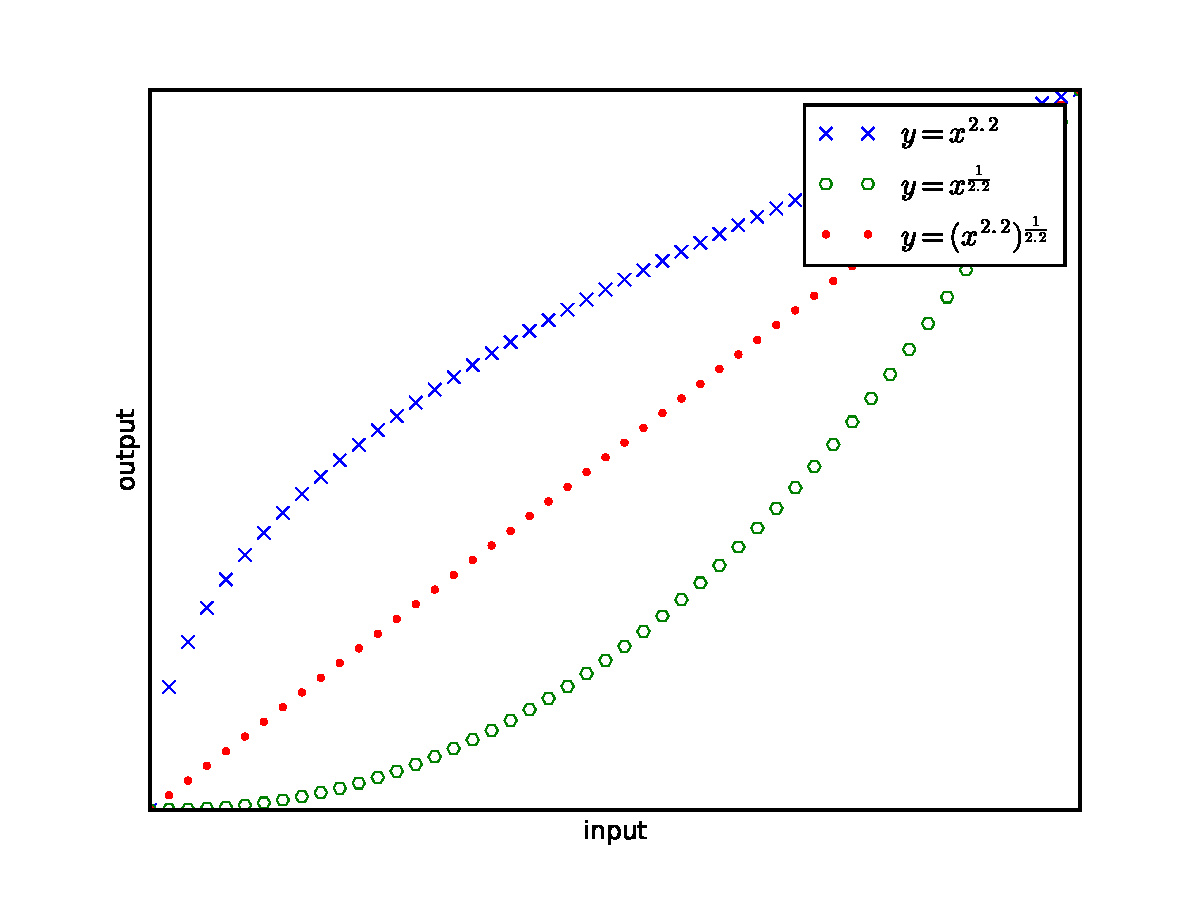
\includegraphics[width=0.5\textwidth]{gamma_coding}
%
%  \caption{Gamma encoding and decoding functions, $\gamma = 2.2$}
%  \label{fig:gamma_coding}
%\end{figure}
\begin{figure}[htb]
  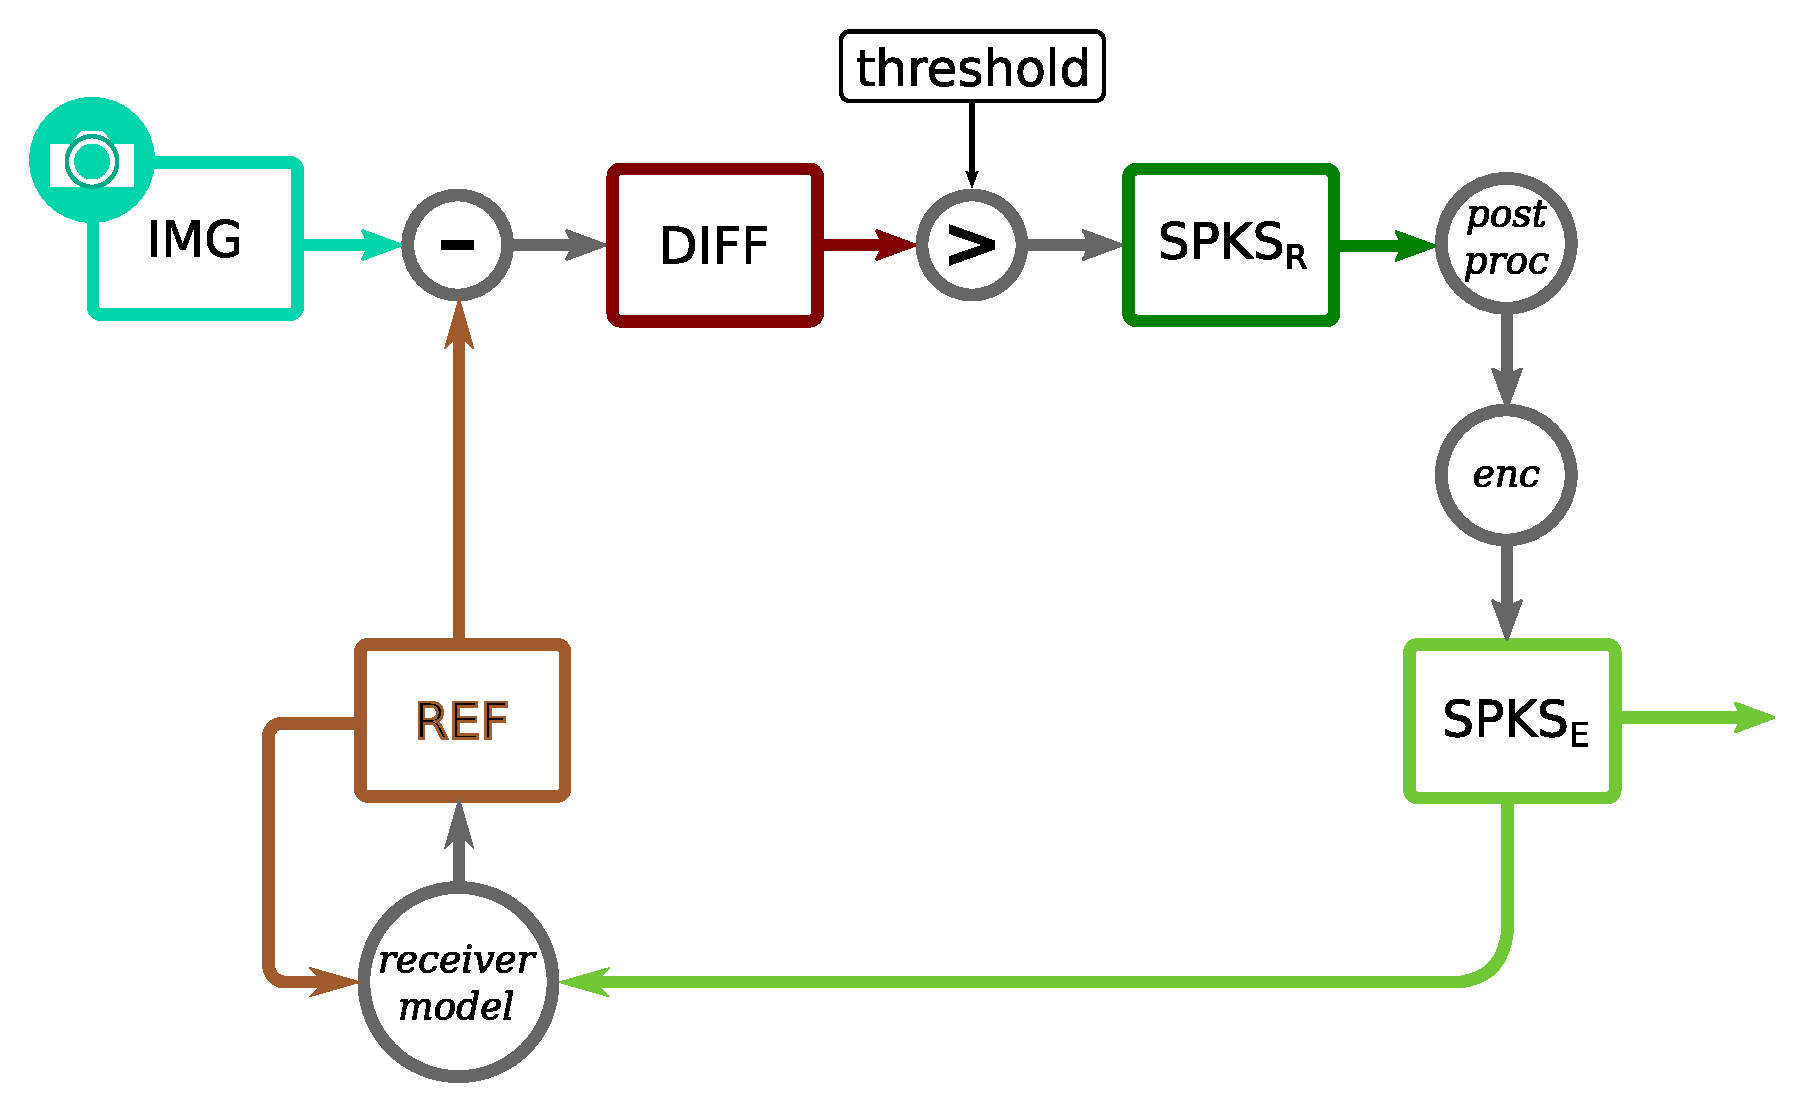
\includegraphics[width=0.5\textwidth]{dvs_emu}
  
  \caption{DVS emulation diagram. Circles indicate operations and rectangles stages of visual information (from frames to spike trains)}
  \label{fig:dvs_emu}
\end{figure}

Figure~\ref{fig:dvs_emu} shows the basic DVS emulation diagram, first asynchronous pixel behaviour is approximated via differencing the current image obtained by the camera and a reference frame. To simulate the spike emission we set a rule, so that whenever a pixel's difference is larger than a certain threshold, we mark that position as ``spiked''. Each spike carries a flag, \textit{up} if there was a positive change in brightness or \textit{down} if a decrease was registered, this can also be thought of as a spike's \textit{sign}. Finally, depending on the selected type of output, we simulate a receiver and update the reference frame accordingly. 


\subsection{Output modes}
\subsubsection{Rate-based}
As in previous emulators\cite{dvs_emu}, the standard output format is rate-based. To calculate the number of spikes that represents a change in brightness we use the following expression
\begin{equation}
  \label{eq:num_spikes_rate}
  N_{H} = \left\lfloor \mathrm{min}\left( T, \;\; \frac{\Delta B}{H} \right) \right\rfloor
\end{equation}
where $N_{H}$ is the number of spikes needed to represent the change in intensity $\Delta B$ in terms of the threshold $H$. Notice that the maximum time ($T$) to transmit all the spikes for one frame is bound by the frame rate of the camera~$(fps)$. If it's only possible to send one spike per millisecond, then $T = 1000/fps$. At this stage we model a perfect receiver, so the update rule for the reference is
\begin{equation}
  \label{eq:ref_update}
  R_{now} = R_{last} + N_{H}\cdot H
\end{equation}

\subsubsection{Time-based}
In its worst case rate-based encoding can send a spike per millisecond per pixel, which can potentially saturate communication channels. One way to prevent this is to encode the value that each spike represents in the time it is sent.

First we propose to linearly encode the number of thresholds exceeded. To do this the result of Equation~\ref{eq:num_spikes_rate} should be interpreted as a bin number $B$ (if a $1 ms$ bin width was used). As in the previous case the time to send all spikes for the current frame is at most $N_{b}=T/W_{b}$, which means the maximum difference possible is $T\cdot H$.

Figure~\ref{fig:linear_time} shows the value-to-spike-time relation, in our proposal earlier spikes represent larger changes in intensity. The main advantage of this encoding is that a single spike could represent multiple rate-based spikes, though the encoded values are limited by time resolution and the frame rate of the camera.

\begin{figure}[htb]
  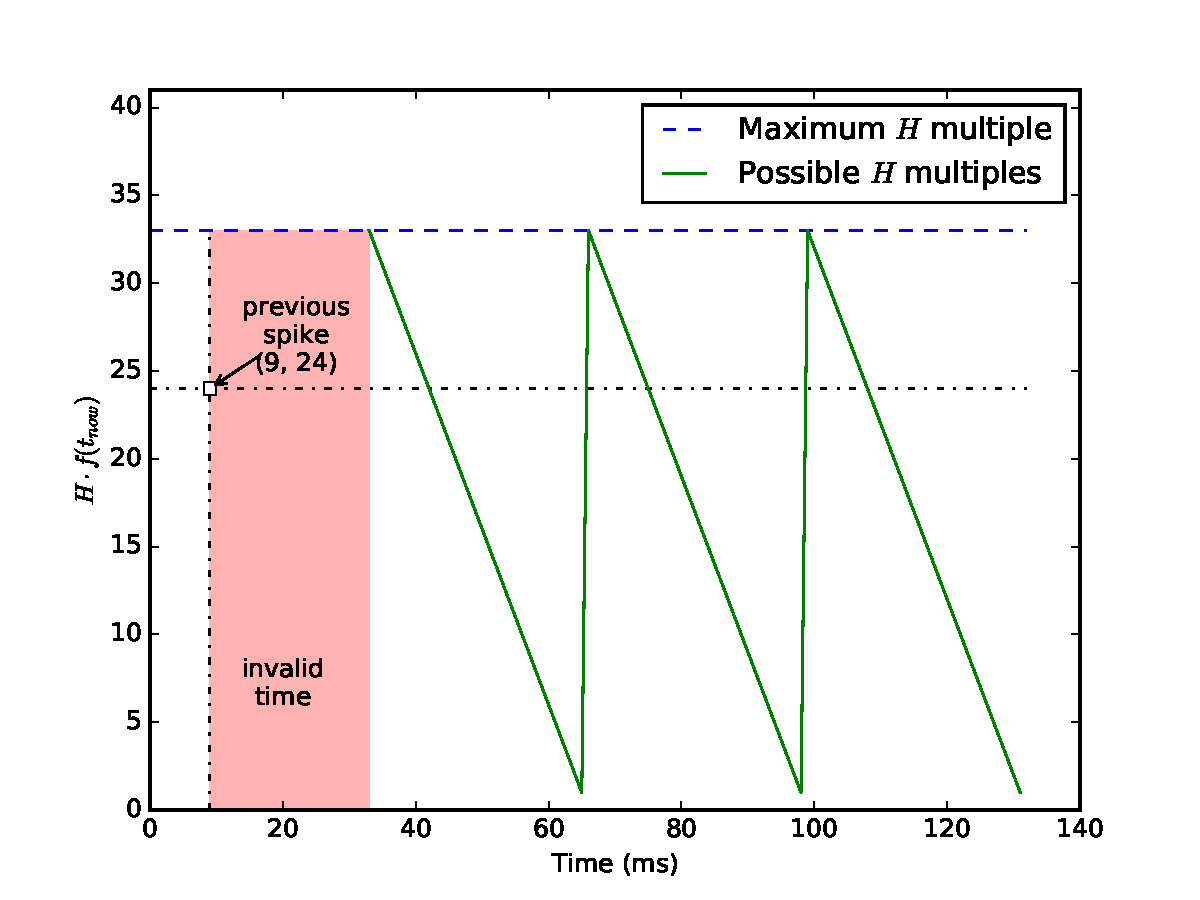
\includegraphics[width=0.5\textwidth]{spike_values_linear}

  \caption{Linear time-based encoding of thresholds ($H$) exceeded}
  \label{fig:linear_time}
\end{figure} 

To decode the spikes on the receiver end, we must keep track of the time and value from the last collected spiked. Let $\Delta t$ be the difference in arrival time between the previous and current spike~(Eq. \ref{eq:time_diff})

\begin{equation}
\Delta t = t_{now} - \left( t_{last} - \left[N_{b} - N_{H}^{last}W_{b} \right] \right)
\label{eq:time_diff}
\end{equation}
where the subtraction of $N_{b} - N_{H}^{last}W_{b}$ sets the time reference to a multiple of time period $T$. We now divide the time difference by the time-bin width to obtain the current bin
\begin{equation}
B = \frac{\mathrm{mod}\left(\Delta t, \;\; T\right)}{W_{b}}
\label{eq:bin_compute}
\end{equation}
here, `$\mathrm{mod}$' calculates its arguments division remainder. Now that the time bin $B$ is known, all it takes to compute the number of thresholds exceeded is
\begin{equation}
 N_{H}^{now} = \left\lfloor N_{b} - B \right\rfloor
 \label{eq:new_Nh_linear}
\end{equation}

%and reduce the probability of getting the wrong value
To mitigate the limitation on maximum encoded values  we propose \textit{binary encoding} of the number of thresholds exceeded. The main advantage of this technique would be to achieve large values with fewer time bins as the growth is exponential (Fig. \ref{fig:exponential_time}). We propose to use this encoding in two ways: \textit{shoot-and-refine} and \textit{full value}. 

\begin{figure}[htb]
  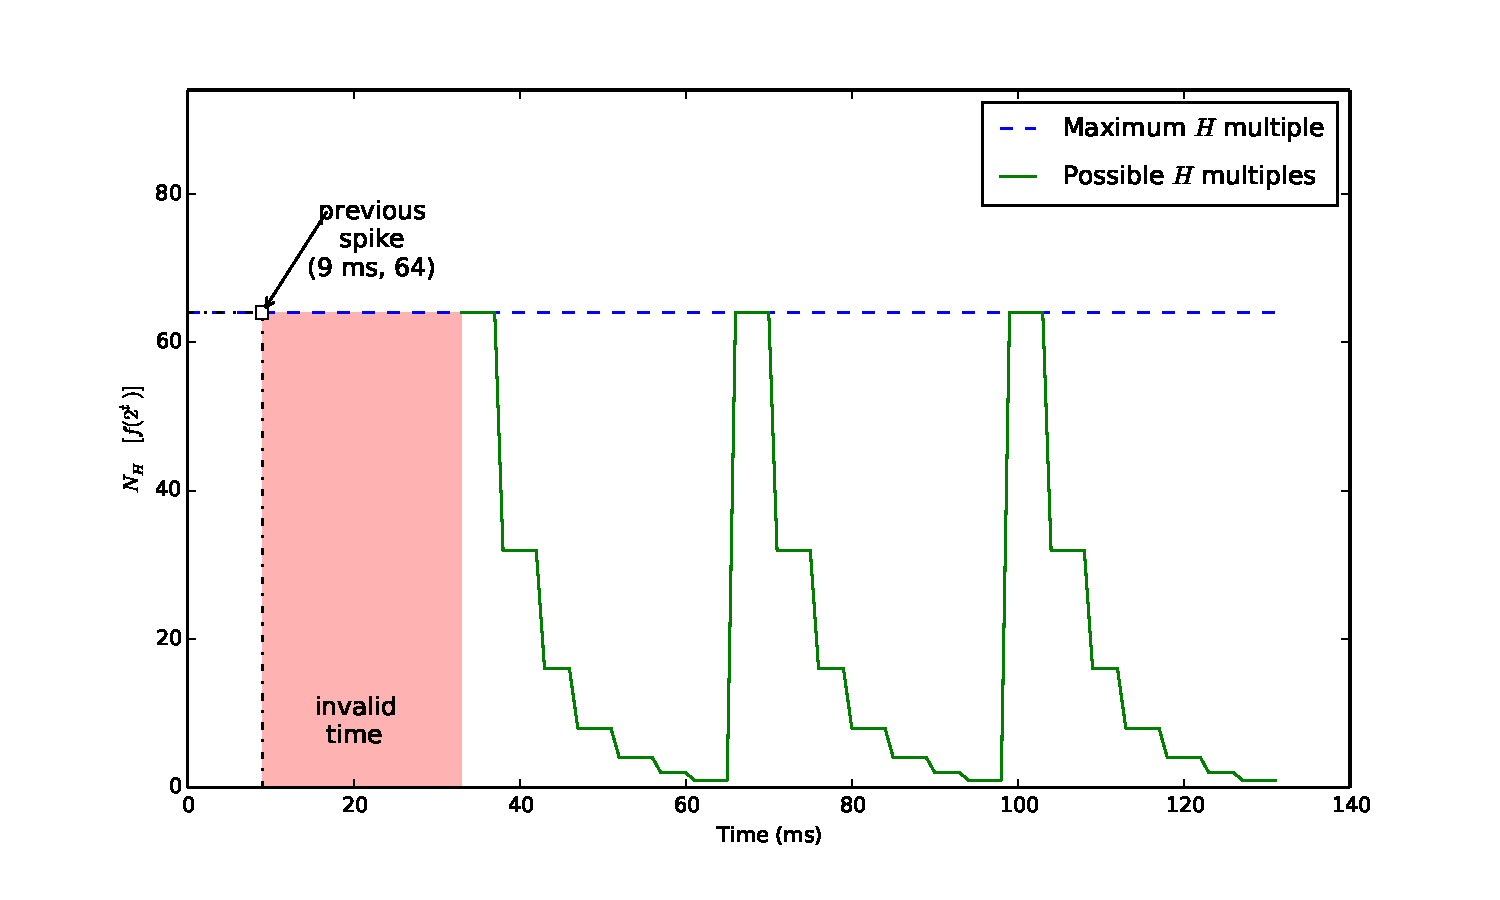
\includegraphics[width=0.5\textwidth]{spike_values_exp}

  \caption{Exponential time-based encoding of thresholds ($H$) exceeded}
  \label{fig:exponential_time}
\end{figure} 

In the \textit{shoot-and-refine} mode, a single spike is sent with an over- or underestimate of the desired value (e.g. the next power of two), and in the following frames we send at most one spike to refine the received value towards the desired one. Decoding can be done in a similar way as the linear case, but we divide the available time in $N_{b}$ bins of width is $W_{b} = T/N_{b}$. Now to compute the time difference
\begin{equation}
\Delta t = t_{now} - \left( t_{last} - 2*\left[N_{b} - log_{2}(N_{H}^{last})W_{b} + 1\right] \right)
\label{eq:time_diff_exp}
\end{equation}

Since we are using time bins that are larger than the system's time resolution, the term $N_{b} - N_{H}^{last}W_{b}$ of Eq.~\ref{eq:time_diff} is transformed into
\begin{equation}
 2*\left[N_{b} - log_{2}(N_{H}^{last})W_{b} + 1\right]
\end{equation}

The correct bin is calculated using Eq.~\ref{eq:bin_compute} as in the linear case; finally for the decoded value
\begin{equation}
N_{H}^{now} = 2^{ \left\lfloor N_{b} - B \right\rfloor }
\label{eq:new_Nh_exp}
\end{equation}

For the \textit{full value} mode many spikes would be sent per pixel each frame, thus providing better resolution to the sent value, the downside to this is that an accumulation buffer is needed in addition to the previous spike time and value buffers. Decoding multiple spikes per frame has to be split in two cases: first if the new spike arrives before the current period is finished, then we accumulate its value to the current decoded value; otherwise we replace the contents of the accumulation buffer with the newly decoded value. Figure~\ref{fig:spike_codes} shows the spike representation of an MNIST digit using the proposed encoding mechanisms.

\begin{figure}[htb]
  \captionsetup[subfigure]{justification=centering}
  
  \centering
  \begin{subfigure}[b]{0.25\textwidth}
    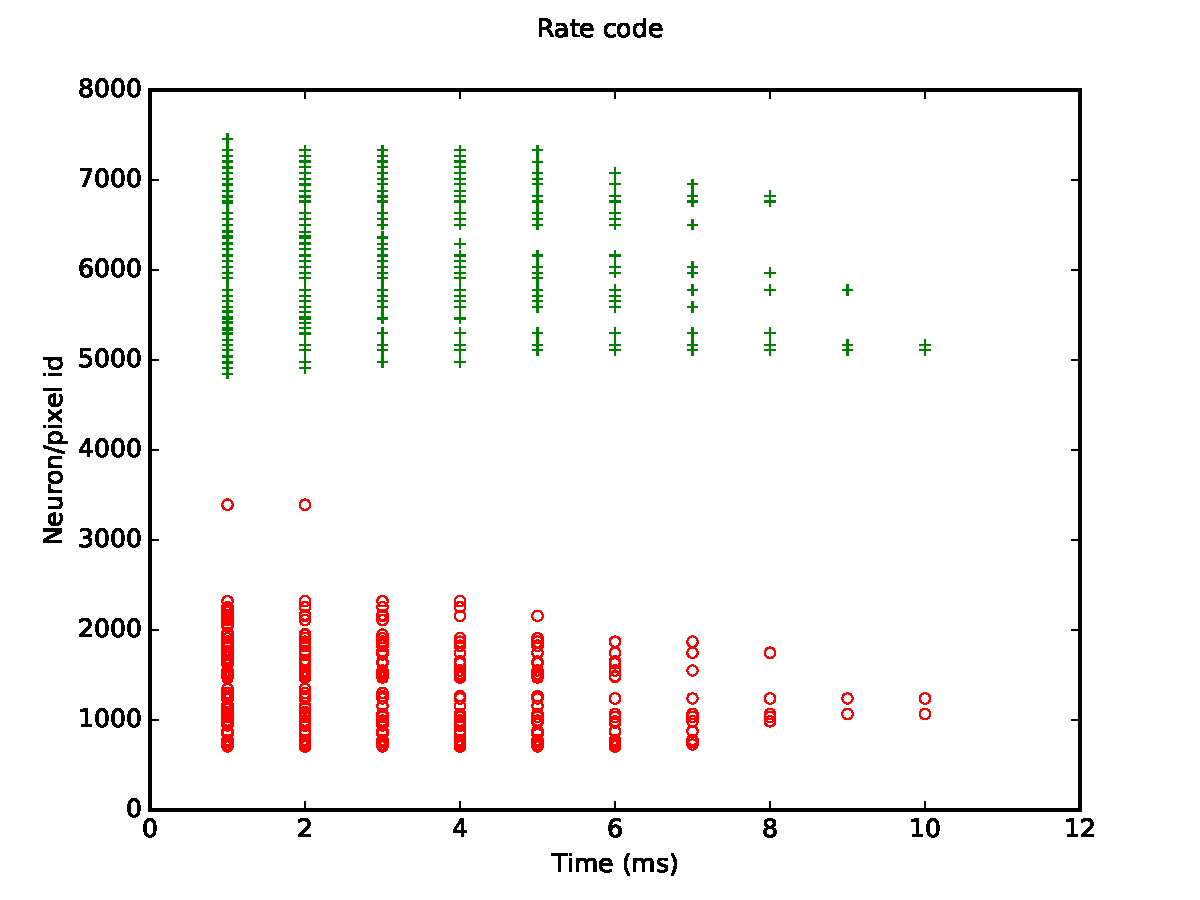
\includegraphics[width=\textwidth]{rate_code}
    \caption{Rate coded spikes.\\ .}
    \label{fig:rate_spikes}
  \end{subfigure}~
  \begin{subfigure}[b]{0.25\textwidth}
    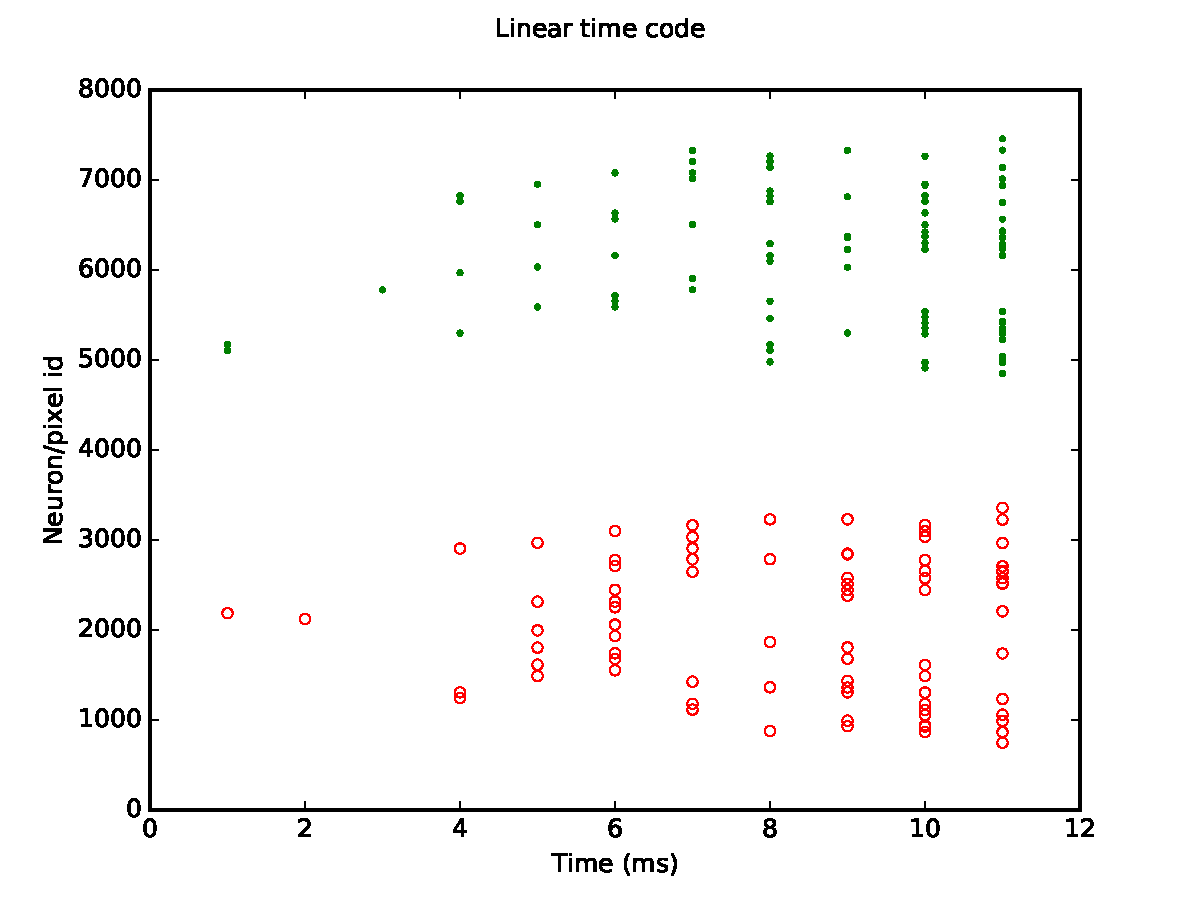
\includegraphics[width=\textwidth]{time_code}
    \caption{Time coded\\spikes (linear).}
    \label{fig:time_spikes}
  \end{subfigure}\\
  \begin{subfigure}[b]{0.25\textwidth}
    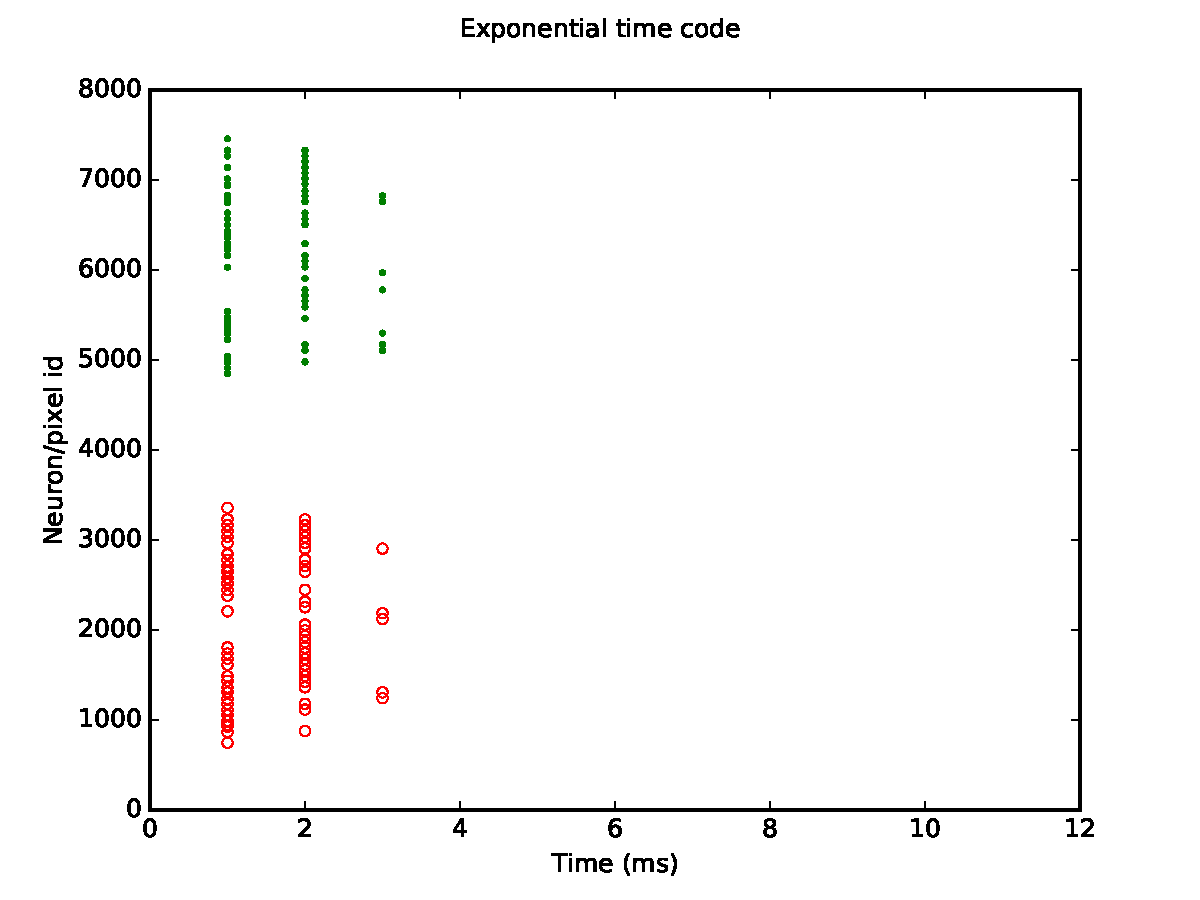
\includegraphics[width=\textwidth]{exp_time_code}
    \caption{Time coded spikes \\(exponential).}
    \label{fig:time_exp_spikes}
  \end{subfigure}
  
  \caption{Difference between spike encodings for the first presentation of an MNIST digit.}
  \label{fig:spike_codes}
\end{figure}

\subsection{Additional behaviours}

In this segment we describe modifications done to the basic DVS emulator, these changes are rendered in Figure~\ref{fig:dvs_emu_inh}. A history decay mechanism was added to the receiver model, constant threshold has been exchanged by an adaptive version, and an inhibitory block (\textit{\textsf{max}}) completes the list of changes.

\begin{figure}[htb]
  
  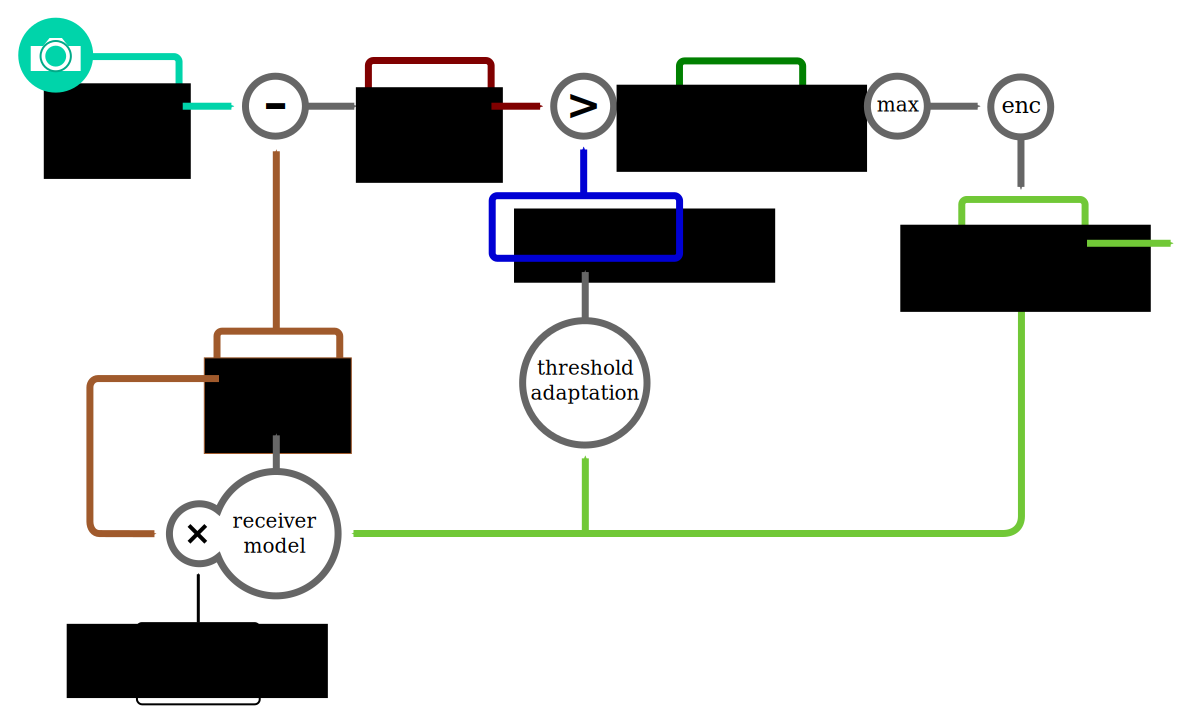
\includegraphics[width=0.5\textwidth]{dvs_emu_decay_adapt_inh}
  \caption{DVS emulation with adaptive thresholds, local inhibition and history decay.}
  \label{fig:dvs_emu_inh}
\end{figure}

\subsubsection{History decay} % - What if spikes get lost?}

Initially we described a system where every spike that is sent will be captured on the receiver end, but this is not always the case. To cope with the latter cases, we now introduce a history decay mechanism which will allow the receiver to, in the long term, recover from missing spikes. Let $D \in \mathbb{R} = (0, 1]$ be the weight history has to calculate the new reference value, then the reference's update rule becomes
\begin{equation}
\label{eq:ref_update_decay}
R_{now} = D\cdot R_{last} + N_{H}\cdot H
\end{equation}

%\begin{figure}[htb]
%  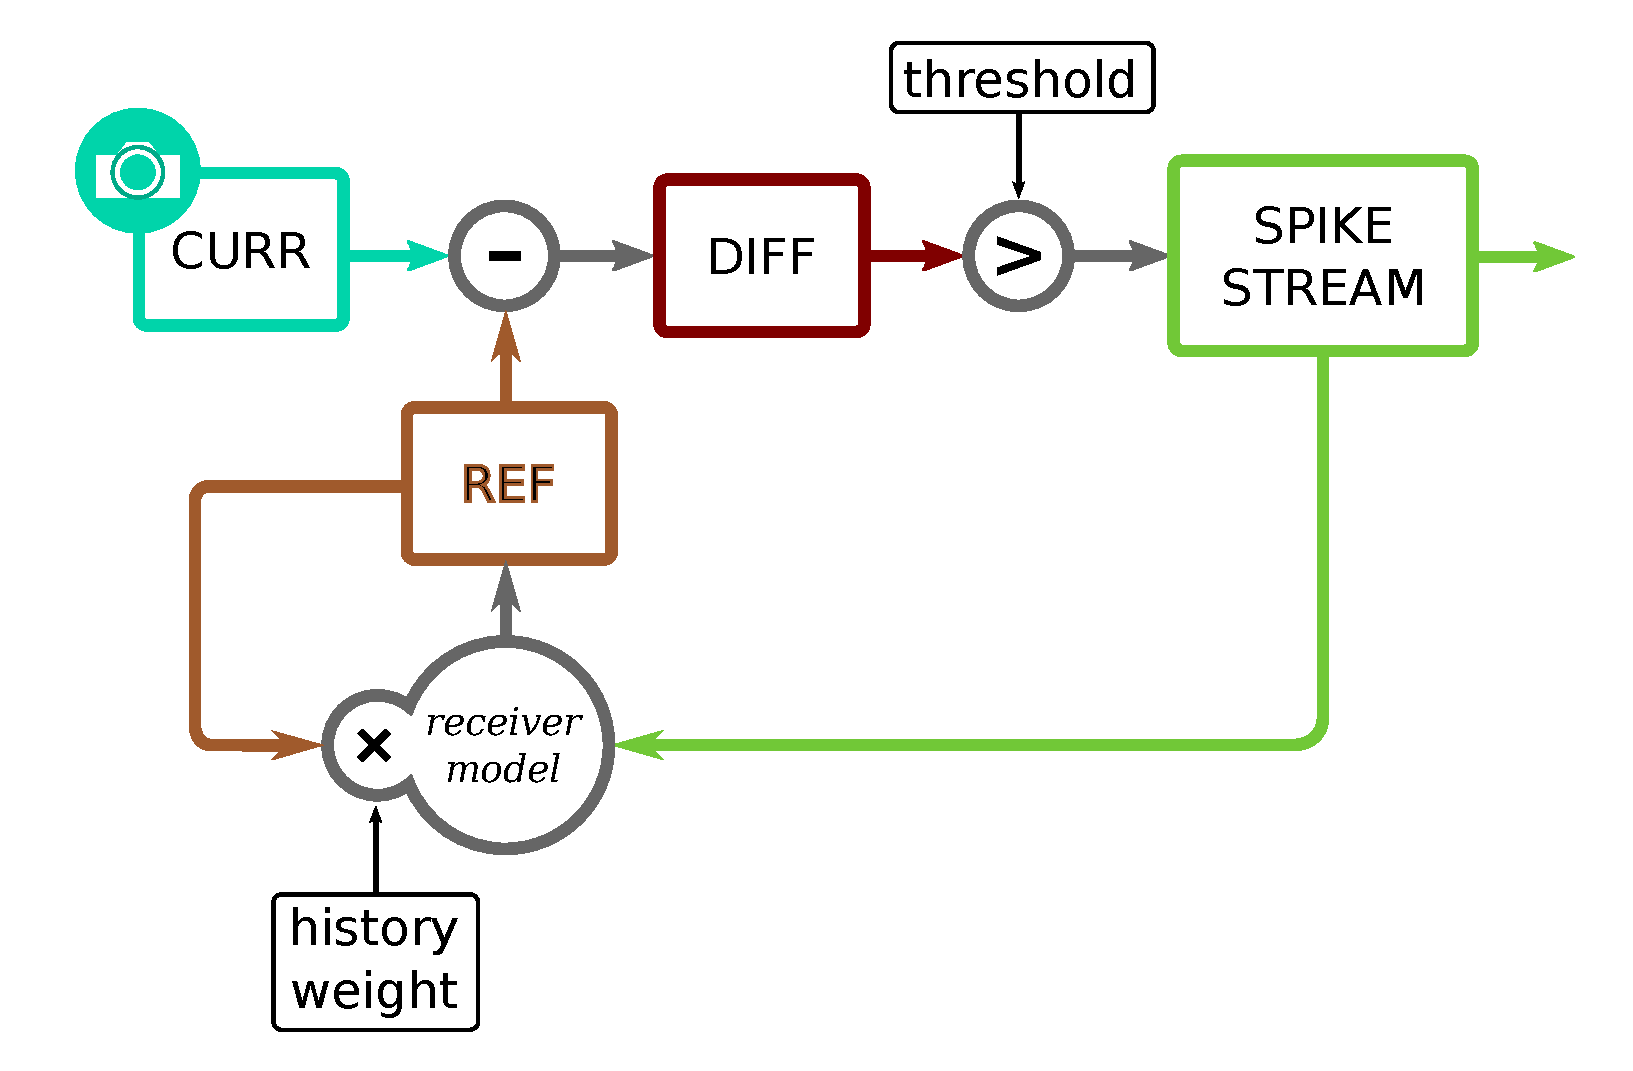
\includegraphics[width=0.5\textwidth]{dvs_emu_decay}
%
%  \caption{DVS emulation with history decay.}
%%  \label{fig:dvs_emu_decay}
%\end{figure}

\subsubsection{Adaptive threshold} 
A subtle detail that other emulators have not captured is the slow-changing pixels, cameras would capture these as similar values in each frame thus the difference would never be enough to generate a spike. Meanwhile in a real DVS pixels receiving insufficient light to immediately trigger a spike, still gain some charge and, after some time, will generate a spike event. We propose to mimic this behaviour by adapting the threshold in a per-pixel basis, that is reduce it if a pixel did not create a spike. Since thresholds value may lowered, they also have to be increased if a spike was generated. These changes in the threshold effectively add a low-pass filter to the system. 

%\begin{figure}[htb]
%
%  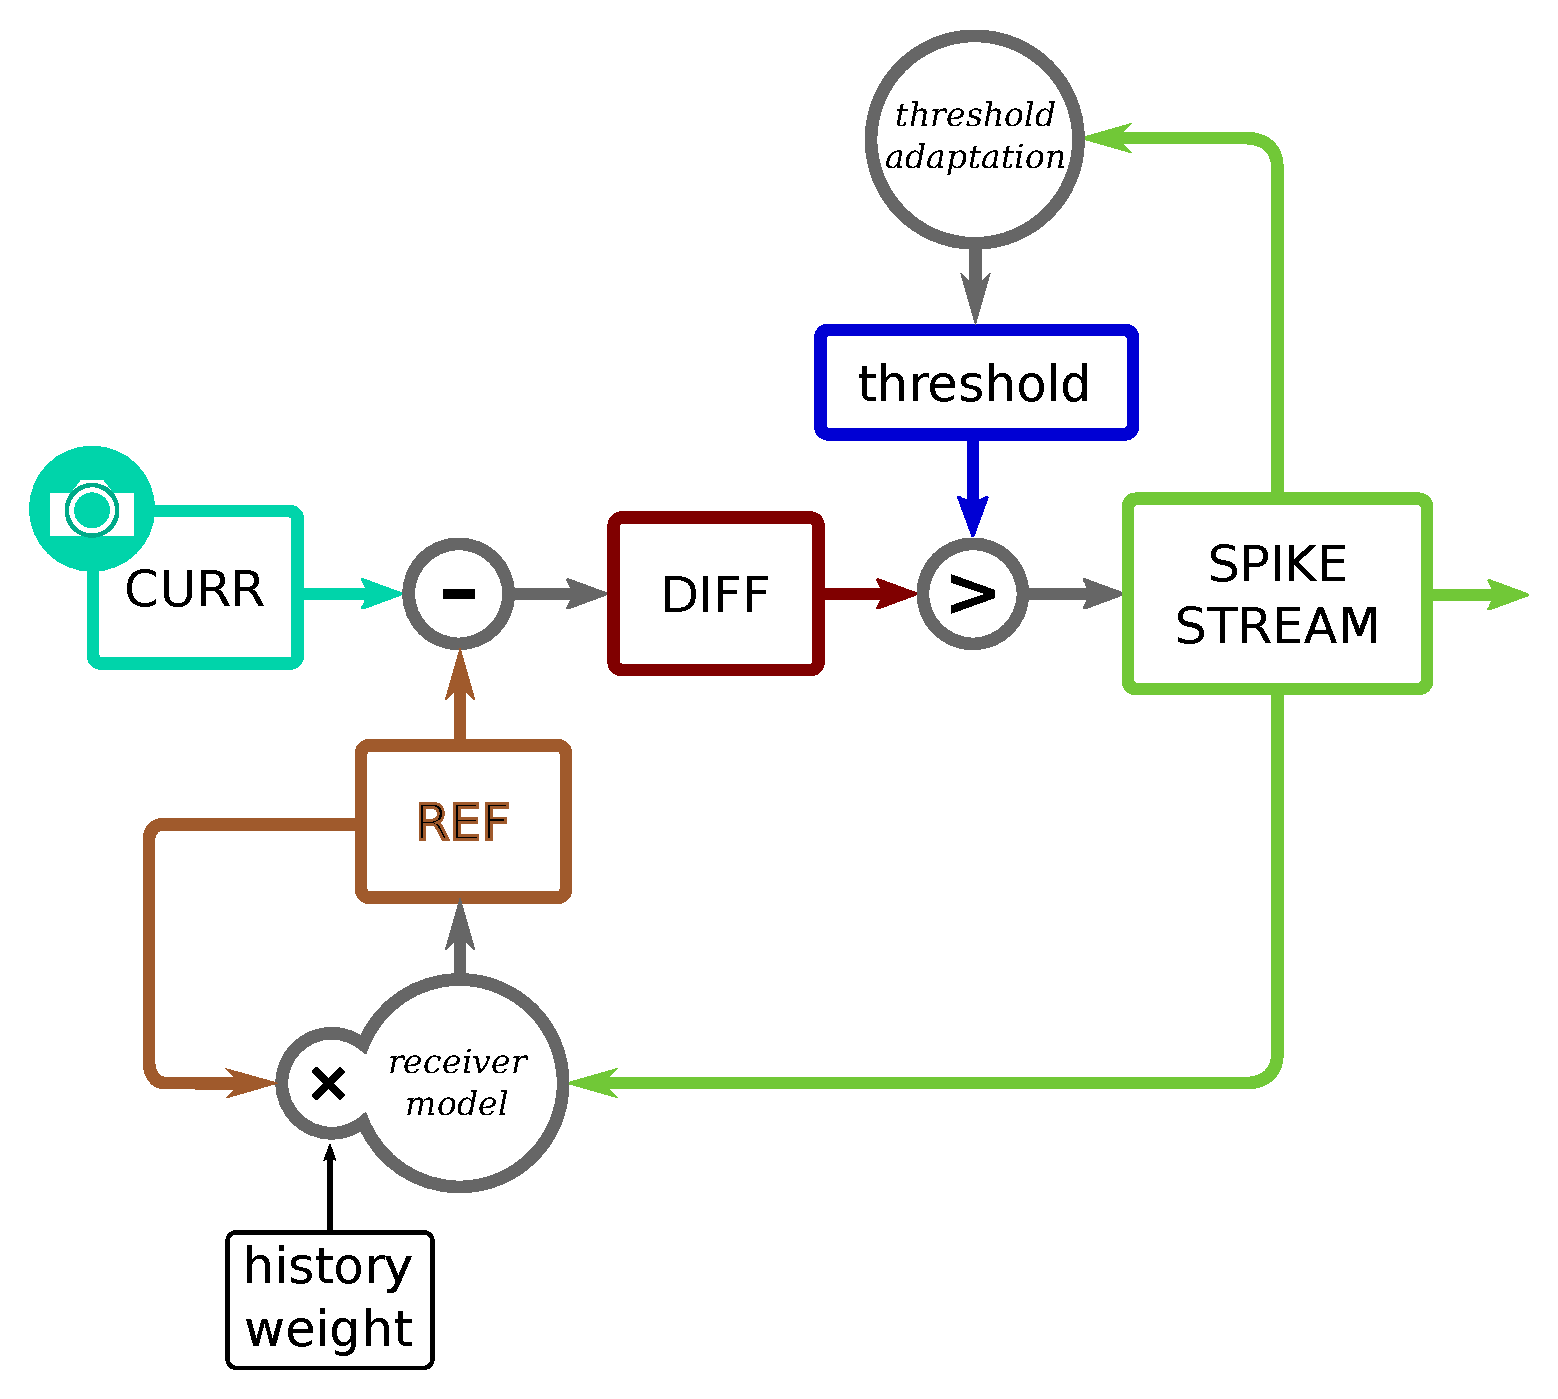
\includegraphics[width=0.5\textwidth]{dvs_emu_decay_adapt}
%  \caption{DVS emulation with adaptive thresholds.}
%  \label{fig:dvs_emu_adapt}
%\end{figure}
\begin{figure}
  \centering
  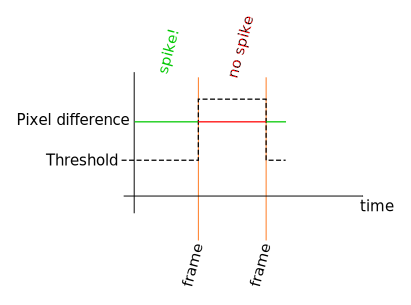
\includegraphics[width=0.3\textwidth]{adaptive_thresh}
  \caption{Adaptive threshold behaviour.}
  \label{fig:adpt_thresh}
\end{figure}

\subsubsection{Local inhibition} 
In mammalian retinas inhibitory circuits play an important role. Some researchers have suggested that it reduces the number of spikes needed to represent what the eye is sensing~\cite{basab}. Our emulator's inhibition mechanism follows a similar idea, since neighbouring pixels have similar values, we suppose that they are transmitting redundant information. The inhibitory behaviour is simply a local MAX operation (similar to complex cells in the HMAX model~\cite{riesenhuber1999hierarchical}) of pixel areas. An example is shown in Figure~\ref{fig:local_inh}, the maximum value (in green; 77) will generate a spike, while other values (in red; 0, 31, and 15) are blocked.

\begin{figure}[htb]
\centering
    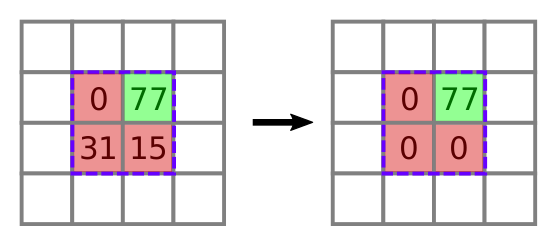
\includegraphics[width=0.3\textwidth]{inh_local_max_img}
    \caption{Local inhibition mechanism, quantities represent the absolute value of the difference between an image and reference.}

  \label{fig:local_inh}
\end{figure}

\section{Results}

The emulator was developed and tested in a desktop computer (Intel i5, 8GB RAM) using the Python and Cython programming languages. We targeted a maximum $128\times 128$-pixel resolution, which can perform at a 60 FPS [lower resolutions (64, 32 and 16 pixel) are also available, and can run at higher frame rates]. This project is open source and it's available at \url{https://github.com/chanokin/pyDVS}.

The initial goal was to provide an alternative for computational neuroscientists that required visual input but could not afford a real DVS. To test the emulators compatibility with neuromorphic hardware, we created a PyNN-compatible~\cite{pynn} code template that communicates to the SpiNNaker platform~\cite{spinnaker_overview} over Ethernet; it can natively encode videos and we provide a ``virtual camera'' that simulates movement on images so they can also be perceived. Using the virtual camera and the MNIST hand-written digits~\cite{mnist} we demonstrate the emulator's behaviours.

\missingfigure{DVS vs EMUlator VISUAL comparison}


The inhibitory behaviour will reduce the amount of spikes that the emulator produces, while keeping some of the information needed to represent the visual input. Figure~\ref{fig:pre_inh} shows the detected spikes as the digit traverses to the right, after the inhibition step fewer spikes remain while keeping the overall shape~(Fig.~\ref{fig:post_inh}).

\begin{figure}[htb]
  \captionsetup[subfigure]{justification=centering}
  \centering
  \begin{subfigure}[b]{0.23\textwidth}
    
\includegraphics[width=\textwidth]{pre_inh_frame_262}
    \caption{Raw spikes.}
    \label{fig:pre_inh}
  \end{subfigure}
  ~
  \begin{subfigure}[b]{0.23\textwidth}
    
\includegraphics[width=\textwidth]{post_inh_frame_262}
    \caption{Inhibited spikes.}
    \label{fig:post_inh}
  \end{subfigure}

  \caption[Difference between raw and local inhibited spikes from a traversing image (inverted images).]{Difference between raw and local inhibited spikes from a traversing image (inverted images\footnotemark ).}
  \label{fig:inh_diff}
\end{figure}
%%%%%%%%%%%%%%
\footnotetext{Notice that most images in the tests are shown inverted. They originally where white over black and are now altered to black over white to better capture the behaviour}
%%%%%%%%%%%%%%

Although the majority of neuromorphic communications are fire-and-forget~\cite{Rast2015}, we were concerned that some information may be lost during transmission and so a history decay mechanism is included to cope with this problem. An example of how both sides of the transmission line can recover from a loss of spikes is shown in Figure~\ref{fig:history_decay}; of particular interest are the $sender$ and $receiver$ rows, which show what both ends ``see''. The leftmost column illustrates how the system starts and what spikes are going to be sent. If some of the spikes are lost (second column) we cannot reconstruct the picture correctly on the receiver end. After 40 waves of spikes (rightmost column), the absolute difference ($|send-recv|$ row) between the images from both ends has pixels whose average value is 8; this means that the missing information has been retransmitted due to history decay. Another effect of this mechanism is that the need to constantly move the image is no longer needed since the reference image's value tend to zero.

\begin{figure}[htb]
%  \captionsetup[subfigure]{justification=centering}
  \centering
  
  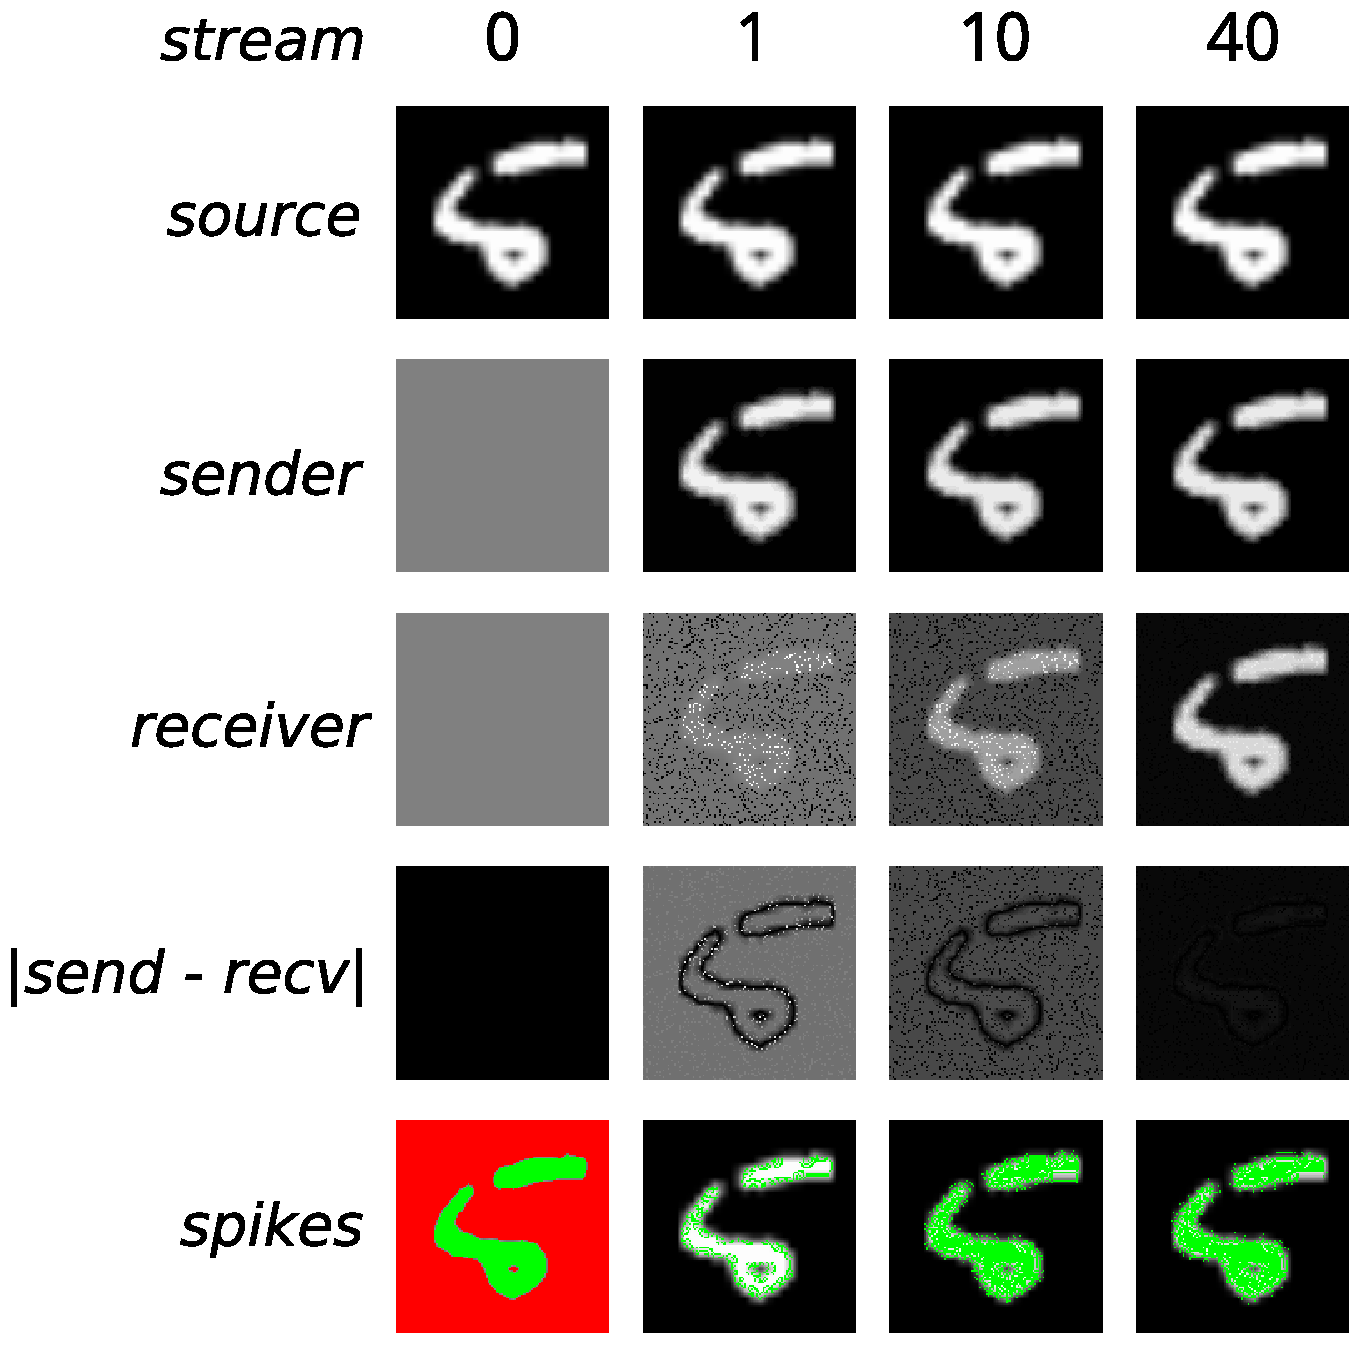
\includegraphics[width=0.45\textwidth]{history_decay}
  \caption{History decay helps to remove transmission errors (1 spike per pixel with linear time encoding).}
  \label{fig:history_decay}
\end{figure}


\section{Conclusion}

An important contribution of the field of computer vision research has been the development of image and video databases. In order to utilize them in spiking neural networks without pointing a real DVS at a monitor, we developed the emulator presented here. Utilising well known datasets, allows an easier comparison between spiking and traditional neural networks.

Emulating a DVS provides the flexibility to modify the system's behaviour in software. One of such changes is to utilize time-encoded spikes, which can aid to break the first barrier to study networks that utilize this method of spike encoding.

\section{Future work}

While the image resolution of the current version of our emulator is low, we've developed an OpenCL version. By using the parallel processing nature of Graphics Processing Units it was possible to encode images at higher resolutions\footnote{We tested up to 1080p video at 30 FPS}; the main problem with this large imagery is that serializing and transmitting such quantities of spikes has proven a hard task.

Research on encoding spikes using convolution kernels is ongoing. We've explored using a kernel based on Carver Mead's original silicon retina~\cite{Mead1989} connectivity and biologically inspired difference of Gaussian kernels~\cite{basab}. These types of encoding could prove to be more efficient as a single spike would represent a region of the image instead of a single pixel.

\printbibliography
%\end{multicols}
\end{document}
